% ML4H 2026 Proceedings Track -- JMLR/PMLR template
% Requires jmlr.cls (from the ML4H template package) in this directory.
\documentclass[pmlr,twocolumn,10pt]{jmlr}

% REQUIRED by the official ML4H 2026 class.
% Valid main-track values include proceedings and findings.
\mlhtrack{proceedings}

% Review/camera-ready switch. Keep \finalfalse for double-blind review.
\newif\iffinal
\finalfalse
% \finaltrue % Uncomment only after acceptance.

\iffinal
  % Replace XXX with the PMLR volume supplied after acceptance.
  \ifmlhneedspmlr
    \jmlrvolume{XXX}
    \jmlryear{2026}
  \fi
  \jmlrworkshop{Machine Learning for Health (ML4H) 2026}
\else
  \jmlrproceedings{}{Submitted to ML4H 2026: \mlhtrackname}
  \jmlrworkshop{Machine Learning for Health (ML4H) 2026}
\fi

% Auto-loaded by jmlr: amsmath, amssymb, natbib, graphicx, url, algorithm2e
\urlstyle{same}
\usepackage{booktabs}
\usepackage{siunitx}
\usepackage[switch]{lineno}

% Architecture figure (TikZ). Compiles with pdfLaTeX.
\usepackage{tikz}
\usetikzlibrary{arrows.meta, positioning}

% Equal-contribution helper (from template)
\newcommand{\equal}[1]{{\hypersetup{linkcolor=black}\thanks{#1}}}

\title[Faithful but Invalid]{Faithful but Invalid: A Statistical-Validity
Firewall for a Governed Single-Cell Senescence Analysis Agent}

% Add names, affiliations, emails, and contribution notes only after acceptance.
\author{Anonymous Author(s)}

% Line numbers are required for review and removed for the camera-ready version.
\iffinal\else\linenumbers\fi

\begin{document}

\maketitle

\begin{abstract}
Large language model (LLM) agents increasingly automate single-cell RNA-seq
analysis. Existing systems verify execution, biological plausibility, or factual
support, but to our knowledge none treat statistical admissibility as a
deterministic precondition for execution or propagate inference states into the
user-facing claim. We show this gap has real consequences. At the \textit{method} level, per-cell differential-expression
testing produces hundreds to thousands of false discoveries under constructed
nulls. In an end-to-end agent pilot, an ungoverned ablation overclaims even when
both arms receive identical pseudobulk DESeq2 outputs. We evaluate at two levels.
At the \textit{method} level, using the constructed-null method of
\citet{squair2021} across five Tabula Muris Senis tissues and 13 cell types,
per-cell testing yields a false discovery on every null split (mean 1{,}425 false
genes at FDR${<}0.05$; truth${=}0$), while pseudobulk testing averages 0.47. At
the \textit{agent} level, across 78 matched donor-split allocations with
identical pseudobulk DESeq2 results supplied to both arms, the governed system
licenses no inferential claims (0/78) and withholds all gene-level results,
while the ungoverned ablation overclaims in 72/78 allocations (92.3\%).
External validation on OneK1K human monocytes (454 donors, 10x Chromium)
confirms calibration (0/10 null allocations with FDR discoveries) and
selectivity (95.5\% recovery of semi-synthetic injected effects, 100\%
direction agreement). Governance is selective: on a real aging contrast
(TMS spleen B cells, 24m vs.\ 3m, 10 biological samples), the governed
path recovers 2{,}246 differentially expressed genes---88.8\%
donor-stable---with 100\% effect-direction agreement among 1{,}167 jointly
significant genes. Multiple-testing correction does not rescue the per-cell
path; the fix is the statistical \textit{unit}. We introduce
a two-gate validity firewall: a deterministic \textit{admissibility} gate that
blocks inadmissible inferences before execution, and a \textit{justification}
gate that withholds conclusions unsupported by the data.
\end{abstract}

\begin{keywords}
single-cell RNA-seq, LLM agents, pseudoreplication, statistical validity, agent
governance, cellular senescence, differential expression
\end{keywords}

\paragraph*{Data and Code Availability}
This study uses publicly available datasets and collects no new data: the
Tabula Muris Senis FACS-processed tissue atlases~\citep{tabulamuris2020} (mouse
aging; biological replicates are individual mice), used for the
constructed-null and positive-control experiments; OneK1K~\citep{yazar2022}
(human PBMCs; ${\sim}980$ donors, 10x Chromium), used for external
calibration and semi-synthetic positive controls; and GSE226225
(WI-38 human fibroblasts with experimentally induced senescence), used as
secondary biological validation. All datasets were obtained from public
repositories. Code and experiment artifacts are provided in anonymized
supplemental materials. The public repository will be released upon acceptance.

\paragraph*{Institutional Review Board (IRB)}
This work analyzes only publicly available, previously published, de-identified
secondary data (a mouse tissue atlas and a human cell-line dataset) and does not
constitute human-subjects research; it therefore does not require IRB approval.

\section{Introduction}
\label{sec:intro}

Single-cell RNA sequencing (scRNA-seq) resolves cell-type-specific responses to
perturbation, and a growing number of LLM agents now automate its analysis
end-to-end~\citep{xiao2024cellagent,scpilot2026,biomni2025}. These agents plan
analyses, call bioinformatics tools, and narrate results in natural language.
Existing systems primarily verify execution, biological plausibility, factual
support, or task completion~\citep{geneagent2025,scagentbench2026}. We are not
aware of prior single-cell agents that represent statistical admissibility as a
deterministic precondition for execution and propagate that state into an
explicit license governing the user-facing inferential claim.

The gap matters because scRNA-seq analysis has a well-documented failure mode: \textit{pseudoreplication}. Cells from the same biological replicate (mouse or donor) share variation that makes them non-independent; treating them as independent inflates the effective sample size and produces false discoveries at scale~\citep{squair2021,zimmerman2021}. The textbook fix is to aggregate to per-replicate ``pseudobulk'' profiles before testing, but this concerns \textit{how the analysis is done}, not whether an artifact was produced. An agent can run a per-cell test, get a real gene list, and report it confidently---without ever checking whether the statistical unit was valid.

We ground our study in \textit{cellular senescence} analysis. The canonical
question a senescence agent faces---does senescence differ between conditions,
ages, or genotypes?---is a between-group differential expression comparison,
and senescence markers such as the SenMayo signature~\citep{saul2022} are
routinely tested per cell, which is the practice that induces pseudoreplication.
Senescence also provides natural ground truth: aging-tissue atlases supply
biological replicates for constructed-null tests, and experimentally induced
senescence datasets offer known senescent-versus-control labels. The governance
mechanism we develop is general to single-cell differential expression;
senescence is simply the domain where we build and validate it.

The practical concern is straightforward. In translational single-cell studies,
differential-expression results inform biomarker panels, patient
stratification, therapeutic-target prioritization, and follow-up perturbation
experiments. A pseudoreplicated gene list can redirect experimental resources
toward associations that do not replicate across patients or biological
samples. Our firewall targets this upstream analytical failure before it is
converted into a biological or translational recommendation. This is already a
known problem for human analysts; an LLM agent that automates the same error
makes it faster and harder to catch.

We ask two questions. First, do agents actually select the invalid analysis path,
and how severe is the resulting error? Second, can a governance layer prevent it
without sacrificing the agent's usefulness?

To answer the first, we use the constructed-null method of \citet{squair2021}:
whole biological replicates are randomly assigned to two synthetic groups so that
no true difference exists, and every reported DE gene is a known false positive.
To answer the second, we build a two-gate validity firewall and show it
prevents the invalid output from becoming a licensed inferential claim.

Our contributions are:
\begin{itemize}
    \item A \textbf{two-gate validity firewall} that converts established
    statistical-design requirements into deterministic, executable governance
    rules for autonomous single-cell agents. Gate~1 (admissibility) blocks
    pseudoreplication, insufficient replicates, and perfect confounding before
    execution; Gate~2 (justification) withholds conclusions the data cannot
    support. No prior single-cell agent, to our knowledge, enforces these
    checks.
    \item A \textbf{method-level quantification} of pseudoreplication failure
    across five tissues and 13 cell types, confirming that per-cell testing
    reports hundreds to thousands of false genes on every null split (mean
    1{,}425 at FDR${<}0.05$), while pseudobulk testing averages 0.47.
    \item A \textbf{same-method governance ablation} isolating the governance
    effect from the statistical method: across 78 matched allocations with
    identical pseudobulk DESeq2 outputs, the governed system overclaims in
    0/78 allocations versus 72/78 ungoverned (92.3\%).
    \item \textbf{External validation on human data}: on OneK1K classical
    monocytes (454 donors), the firewall produces zero false discoveries across
    10 null allocations, recovers 95.5\% of injected effects in semi-synthetic
    positive controls, and achieves 100\% correct admissibility decisions
    across 150 confound-gate challenges.
    \item A \textbf{selectivity demonstration}: the firewall preserves
    sensitivity to real biology, recovering 2{,}246 genes (88.8\%
    donor-stable) on a TMS aging contrast with 100\% direction agreement
    among jointly significant genes.
\end{itemize}

\section{Related Work}

\paragraph{Biomedical analysis agents.}
CellAgent~\citep{xiao2024cellagent}, scPilot~\citep{scpilot2026},
Biomni~\citep{biomni2025}, AutoBA~\citep{autoba2024}, and related systems
automate scRNA-seq and broader biomedical workflows using
planner/executor/evaluator loops. None of these agents enforce pseudobulk
aggregation as a precondition for between-group differential expression:
CellAgent wraps \texttt{scanpy.tl.rank\_genes\_groups} (a per-cell test) and
does not check for a biological-replicate column;
scPilot delegates to generated code without validating the statistical unit;
Biomni operates across modalities but does not distinguish per-cell from
per-replicate testing; AutoBA generates analysis pipelines from natural
language but applies no admissibility gate.
CellVoyager~\citep{cellvoyager2026} is the closest comparator: it
\textit{can} perform pseudobulk aggregation, but only incorporates it
after a human reviewer explicitly requests ``more statistically rigorous''
analysis; pseudobulk is an LLM-chosen improvement, not a deterministic
precondition.
A recent single-cell agent benchmark~\citep{scagentbench2026} evaluates
50 tasks across 18 metrics including program synthesis, execution, knowledge
integration, and robustness.
These capability-oriented evaluations measure whether an agent completes a
task correctly; we complement them by testing whether the design underlying a
completed analysis licenses the inferential claim communicated to the user.
scBench~\citep{scbench2026} and BioDSA-1K~\citep{biodsa2025} similarly measure
agent error rates but do not target pseudoreplication or provide a governance
mechanism.

\paragraph{Evidence-grounded scientific agents.}
GeneAgent~\citep{geneagent2025} extracts biological assertions from gene-set
analyses and verifies them against curated databases, classifying claims as
supported, partially supported, or refuted. EviBound~\citep{evibound2025}
eliminates hallucinated claims by checking that an agent's output is backed by
real artifacts: a queryable run, present files, a completed status. GeneAgent
asks whether a biological statement is supported by external knowledge;
EviBound asks whether a computation happened. Our system asks a different
question: whether the current dataset and study design statistically license
an inferential statement. These are complementary layers---a database may
support that a gene participates in senescence while the current experiment
cannot establish a group difference because donors were pseudoreplicated.

\paragraph{Automated scientific testing.}
POPPER~\citep{popper2025} controls Type-I error across a sequence of
falsification experiments. It asks whether error is controlled
\textit{across} tests; we ask whether a \textit{single} test's statistical unit
is valid---the layer where pseudoreplication lives.

\paragraph{Pseudoreplication in single-cell data.}
\citet{squair2021} demonstrated that single-cell DE methods ignoring
between-replicate variation produce hundreds of false discoveries, and introduced
the constructed-null protocol we adopt. \citet{zimmerman2021} and subsequent
work~\citep{nested2025} formalize pseudobulk and mixed-model corrections. This
literature targets human analysts; we connect it with the agent literature by
converting established statistical-design requirements into executable
governance rules for autonomous biomedical agents.

\section{Methodology}

\begin{figure}[htbp]
\floatconts
  {fig:arch}
  {\caption{The governed pipeline. The LLM (blue) only \emph{proposes} an
  intent; two deterministic gates (red) \emph{dispose}. Gate~1 refuses
  statistically invalid designs before execution; Gate~2 withholds conclusions
  the result cannot support. EviBound would verify that the tool \emph{ran};
  POPPER controls error \emph{across} a sequence of tools; our gates govern the
  validity of the individual inference.}}
  {%
  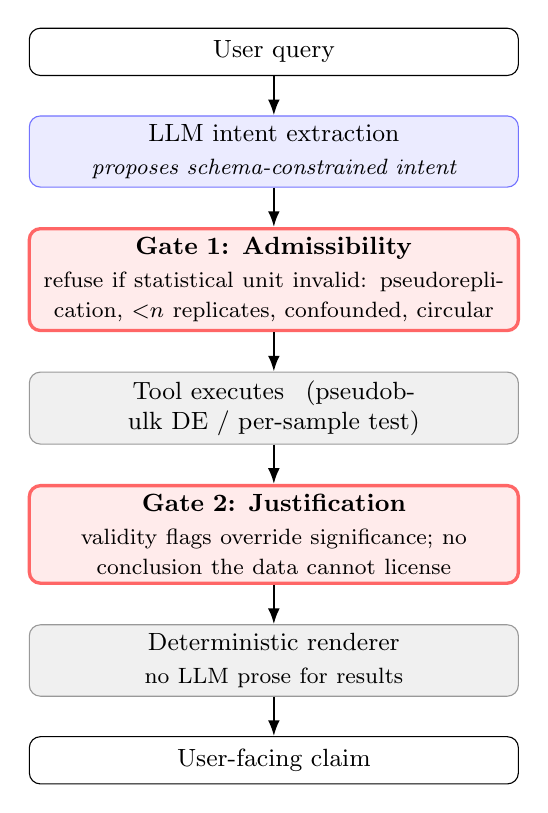
\begin{tikzpicture}[
    node distance=5mm,
    box/.style={draw, rounded corners, align=center, text width=6cm,
                minimum height=6mm, font=\small, inner sep=3pt},
    llmbox/.style={box, fill=blue!8, draw=blue!55},
    gatebox/.style={box, fill=red!8, draw=red!60, very thick},
    detbox/.style={box, fill=black!6, draw=black!40},
    arr/.style={-{Latex[length=2mm]}, thick}
  ]
  \node[box] (q) {User query};
  \node[llmbox, below=of q] (llm)
    {LLM intent extraction\\[1pt]\footnotesize\itshape proposes schema-constrained intent};
  \node[gatebox, below=of llm] (g1)
    {\textbf{Gate 1: Admissibility}\\[1pt]\footnotesize refuse if statistical unit invalid:
     pseudoreplication, ${<}n$ replicates, confounded, circular};
  \node[detbox, below=of g1] (tool)
    {Tool executes \, (pseudobulk DE / per-sample test)};
  \node[gatebox, below=of tool] (g2)
    {\textbf{Gate 2: Justification}\\[1pt]\footnotesize validity flags override significance;
     no conclusion the data cannot license};
  \node[detbox, below=of g2] (rend)
    {Deterministic renderer\\[1pt]\footnotesize no LLM prose for results};
  \node[box, below=of rend] (out) {User-facing claim};
  \foreach \a/\b in {q/llm, llm/g1, g1/tool, tool/g2, g2/rend, rend/out}
    \draw[arr] (\a)--(\b);
  \end{tikzpicture}
  }
\end{figure}

\subsection{Governed Single-LLM Agent}

The agent answers senescence-analysis queries---senescence scoring, marker
coverage, cell-type annotation, and the senescence-difference question between
groups---over an uploaded scRNA-seq dataset. It confines the LLM to a single
non-authoritative role: intent extraction. Routing proceeds in three tiers:
(i)~a deterministic keyword router for common queries; (ii)~an LLM that emits a
schema-constrained intent JSON, validated against the real dataset before
routing; (iii)~an LLM tool-calling fallback. In all tiers the LLM proposes;
two deterministic gates decide (\figureref{fig:arch}). User-facing text is
produced by a deterministic renderer, never by the LLM.

The operation of interest is the senescence-difference question, which the agent
serves in two ways: a per-replicate test on SenMayo scores, or pseudobulk
differential expression on genes. Both are between-group comparisons whose
validity depends on the statistical unit, making them the natural site for the
firewall.

\subsection{Two-Gate Validity Firewall}

\paragraph{Gate 1: Admissibility (pre-execution).}
Before any inferential tool runs, a deterministic check inspects the data
design: does a biological-replicate column exist? Are there enough replicates
per group? Is the contrast confounded? Would the inference be circular? If the
design is inadmissible, the tool never executes and the agent returns the reason.
The minimum-replicate threshold is tool-specific: ${\geq}2$ per group for
score-based tests, ${\geq}3$ for DESeq2 (whose dispersion estimation is
unreliable below three). This blocks pseudoreplication at its source---a per-cell
comparison across replicate-defined groups is refused before a p-value is ever
computed.

\paragraph{Gate 2: Justification (post-execution).}
Every tool result carries an inference state and a set of validity flags
(e.g., \texttt{cell\_unit\_not\_inferential},
\texttt{circular\_inference\_risk},
\texttt{uncorrected\_multiple\_testing}). A validity flag overrides the
significance axis: a result carrying a flag is forced to descriptive-only
regardless of its p-value. We empirically demonstrate pseudoreplication and the
pre-execution checks for replicate sufficiency and perfect confounding. The
circular-inference and uncorrected-multiple-testing flags remain architectural
extension points and are not evaluated here.

\begin{figure}[htbp]
\floatconts
  {fig:endpoints}
  {\caption{Three endpoints that governance separates. Prior agents conflate
  all three: a tool produces output, and the agent reports it as a conclusion.
  Our firewall interposes Gate~2 between raw output and licensed conclusion, and
  a deterministic renderer between licensed conclusion and user reply. On null
  data, the governed path produces raw discoveries (mean 132.8 genes) but
  licenses none and withholds all from the user.}}
  {%
  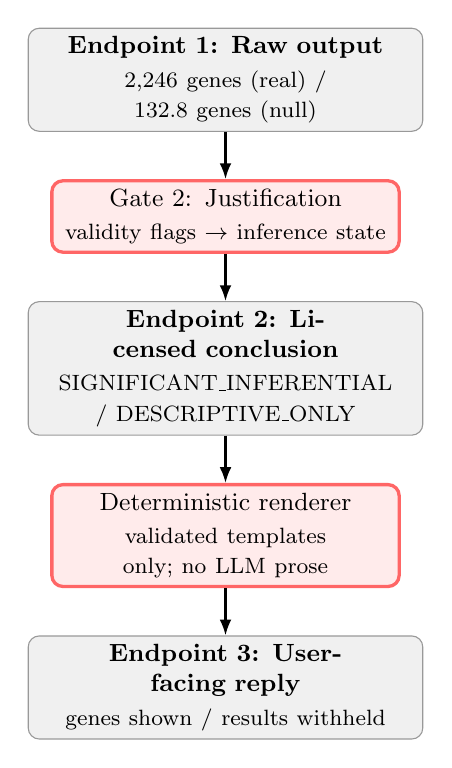
\begin{tikzpicture}[
    node distance=4mm and 8mm,
    box/.style={draw, rounded corners, align=center, text width=4.8cm,
                minimum height=7mm, font=\small, inner sep=3pt},
    endpt/.style={box, fill=black!6, draw=black!40},
    gate/.style={box, fill=red!8, draw=red!60, very thick, text width=4.2cm},
    arr/.style={-{Latex[length=2mm]}, thick}
  ]
  \node[endpt] (raw) {\textbf{Endpoint 1: Raw output}\\[1pt]
    \footnotesize 2{,}246 genes (real) / 132.8 genes (null)};
  \node[gate, below=6mm of raw] (g2) {Gate 2: Justification\\[1pt]
    \footnotesize validity flags $\to$ inference state};
  \node[endpt, below=6mm of g2] (lic) {\textbf{Endpoint 2: Licensed conclusion}\\[1pt]
    \footnotesize SIGNIFICANT\_INFERENTIAL / DESCRIPTIVE\_ONLY};
  \node[gate, below=6mm of lic] (rend) {Deterministic renderer\\[1pt]
    \footnotesize validated templates only; no LLM prose};
  \node[endpt, below=6mm of rend] (usr) {\textbf{Endpoint 3: User-facing reply}\\[1pt]
    \footnotesize genes shown / results withheld};
  \draw[arr] (raw) -- (g2);
  \draw[arr] (g2) -- (lic);
  \draw[arr] (lic) -- (rend);
  \draw[arr] (rend) -- (usr);
  \end{tikzpicture}
  }
\end{figure}

\subsection{Donor-Stability Assessment}

For the positive-control analysis, we assess whether each FDR-significant gene's
effect is robust to donor composition via a leave-one-donor-out procedure. For
each of the $n$ biological samples in the contrast, we remove that sample and
recompute the between-group effect (mean difference of $\log_2(\text{CPM}+1)$
pseudobulk profiles) on the remaining $n{-}1$ samples. A gene is
\textit{donor-stable} if (a)~its effect direction is preserved across all $n$
omissions, and (b)~the minimum retained effect magnitude across omissions is
${\geq}50\%$ of the full-sample effect. This is a deterministic sensitivity
analysis, not a second significance test: DESeq2 is not refitted. The
denominator for the reported stability fraction (e.g., 1{,}995/2{,}246 =
88.8\%) is the number of FDR-significant genes from the full-sample DESeq2 run.

\subsection{Evaluation Design}

We evaluate at two levels, which we report separately throughout:

\paragraph{Method-level (statistical-unit experiment).}
Following \citet{squair2021}, we create a known null by randomly assigning whole
biological replicates (mice) to two synthetic groups within a single cell type.
By construction, no true difference exists; every reported DE gene is a false
positive. On each of $K{=}200$ permutations we run two statistical methods on
log-normalized expression:
\begin{itemize}
    \item \textbf{Per-cell:} Wilcoxon rank-sum over individual
    cells---the pseudoreplication path.
    \item \textbf{Pseudobulk:} per-replicate mean profiles tested
    across replicates.
\end{itemize}
We count false positives at raw $p<0.05$ and at BH-FDR${<}0.05$ (truth${=}0$
in both cases) and report the \textit{null-split false-discovery incidence}: the
fraction of null splits on which a path reports at least one BH-significant gene.

\paragraph{Agent-level (same-method governance ablation).}
We run the governed system and its ungoverned ablation on 78 matched
donor-split allocations across five tissue/cell-type configurations.
Crucially, both arms receive \textit{identical} pseudobulk DESeq2 results:
the same donor allocation, the same design factors, the same significant-gene
sets. The only difference is the governance stack. The aggregator enforces
exact parity on allocation identity, discovery count, significant genes,
design, and covariates; any mismatch is rejected. This isolates the governance
effect from the statistical-method effect. The primary endpoint is
the \textit{overclaim rate}: the fraction of allocations in which the agent's
user-facing reply makes an inferential significance assertion although the
associated tool result is not licensed for inferential reporting. A
deterministic claim linter detects positive significance assertions using a
fixed set of regex patterns (e.g., ``is statistically significant,'' ``evidence
of statistical significance,'' numeric p-value reports), excluding negated
statements such as ``not statistically significant'' and p-value disclaimers
such as ``no p-value from this tool.'' The linter compares detected assertions
with the independently generated tool inference state. A reply is scored as an
overclaim only when a positive assertion is present and that state is not
inferentially licensed. Scoring is deterministic and identical for both
arms; the complete phrase list and unit tests are provided in the
supplement. A reply is scored as
\textit{withheld} if it does not expose the gene-level result table to the user.
Raw discovery counts from the agent pilot are descriptive diagnostics, not
proven gene-level false positives, because residual donor heterogeneity can
produce discoveries even under a null assignment. The governance question is
whether those discoveries are \textit{licensed}.

\subsection{Data}

We use three datasets spanning mouse and human, plate-based and droplet
protocols. Tabula Muris Senis FACS-processed tissues~\citep{tabulamuris2020}
(Smart-seq2; biological replicates = mice; 5 tissues, 13 cell types) for the
constructed-null experiments and positive-control analysis. OneK1K classical
monocytes~\citep{yazar2022} (10x Chromium/UMI; ${\sim}980$ donors, 454
retained per allocation) for external statistical calibration and
semi-synthetic positive controls. GSE226225 (WI-38 human fibroblasts,
etoposide-induced senescence, 3 vs.\ 2 samples) for secondary biological
validation.

\section{Results}

\subsection{Method-Level: Pseudoreplication Produces Mass False Discovery}

\tableref{tab:null} reports the statistical-unit experiment across five tissues
and 13 cell types (200 permutations each). The pattern is consistent: on data
with no real difference, per-cell testing produces a false discovery on every
single null split. The mean number of false genes at FDR${<}0.05$ is 1{,}425,
ranging from 63 (a small B-cell population in liver) to 5{,}748 (hepatocytes,
which have many cells per replicate). The pseudobulk path averages 0.47
false genes, with a mean null-split false-discovery incidence of 2.5\%. Twelve
of 13 configurations are at or below the nominal $\alpha{=}0.05$; collecting
duct epithelium is higher at 9\%. The severity of pseudoreplication scales
with cells per replicate, but its occurrence---a false discovery on every
split---does not vary by tissue or cell type.

\begin{table*}[htbp]
\floatconts
  {tab:null}
  {\caption{Method-level constructed-null experiment across five tissues and 13
  cell types (200 permutations each). Every reported gene is a false positive by
  construction (truth${=}0$). FP = mean false-positive genes at FDR${<}0.05$ per
  null split. Split incidence = fraction of splits reporting ${\geq}1$ DE gene.
  Per-cell testing fails on every split in every configuration. Pseudobulk
  averages 2.5\% split incidence; 12 of 13 configurations are at or below
  5\%.}}
  {\footnotesize
  \begin{tabular}{llrrrrr}
  \toprule
  \textbf{Tissue} & \textbf{Cell type} & \textbf{Mice} & \textbf{Genes} &
  \textbf{Per-cell FP} & \textbf{Pseudobulk FP} & \textbf{Split incid.\ (per-cell / pb)} \\
  \midrule
  Kidney      & proximal tubule epi.        & 7  & 5{,}333 & 916   & 0.0 & 100\% / 1\% \\
  Kidney      & fenestrated                 & 7  & 5{,}867 & 221   & 0.0 & 100\% / 2\% \\
  Kidney      & collecting duct epi.        & 6  & 5{,}176 & 708   & 0.1 & 100\% / 9\% \\
  Liver       & hepatocyte                  & 9  & 9{,}104 & 5{,}748 & 0.7 & 100\% / 1\% \\
  Liver       & hepatic sinusoid endo.      & 6  & 7{,}075 & 1{,}161 & 0.0 & 100\% / 0\% \\
  Liver       & B cell                      & 4  & 4{,}741 & 63    & 0.0 & 100\% / 0\% \\
  Spleen      & B cell                      & 13 & 5{,}514 & 2{,}291 & 0.0 & 100\% / 2\% \\
  Spleen      & CD4 T cell                  & 12 & 5{,}629 & 201   & 0.0 & 100\% / 1\% \\
  Spleen      & CD8 T cell                  & 9  & 6{,}113 & 291   & 0.1 & 100\% / 3\% \\
  Aorta       & aortic endothelial          & 7  & 6{,}007 & 883   & 0.0 & 100\% / 4\% \\
  Limb muscle & satellite cell              & 13 & 5{,}005 & 2{,}877 & 4.9 & 100\% / 5\% \\
  Limb muscle & mesenchymal stem cell       & 12 & 7{,}045 & 2{,}570 & 0.3 & 100\% / 3\% \\
  Limb muscle & endothelial                 & 10 & 4{,}458 & 593   & 0.0 & 100\% / 2\% \\
  \midrule
  \multicolumn{4}{l}{\textbf{Mean}} & \textbf{1{,}425} & \textbf{0.47} & \textbf{100\% / 2.5\%} \\
  \bottomrule
  \end{tabular}}
\end{table*}

\begin{figure}[htbp]
\floatconts
  {fig:null_gap}
  {\caption{Mean false positives (FDR${<}0.05$) per null split across 13
  tissue/cell-type configurations (log scale). Per-cell testing (red) produces
  63--5{,}748 false genes; pseudobulk (blue) produces 0--4.9. Values displayed
  as 0.0 in \tableref{tab:null} are placed at 0.01 solely for visualization on
  the logarithmic axis.}}
  {%
  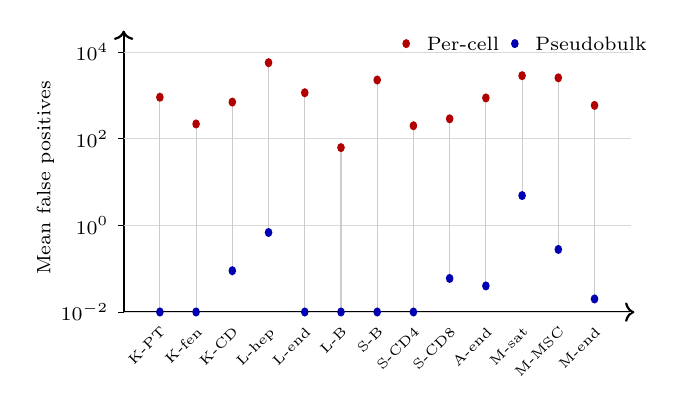
\begin{tikzpicture}[xscale=0.46,yscale=0.55]
  % axes
  \draw[thick,->] (0,0) -- (14.1,0);
  \draw[thick,->] (0,0) -- (0,6.5);
  \node[rotate=90,font=\scriptsize,anchor=south] at (-1.65,3.1)
    {Mean false positives};
  % y-axis ticks: 10^-2 to 10^4
  \foreach \y/\lab in {0/$10^{-2}$, 2/$10^{0}$, 4/$10^{2}$, 6/$10^{4}$} {
    \draw (0,\y) -- (-0.15,\y) node[left, font=\scriptsize] {\lab};
    \draw[gray!30, thin] (0,\y) -- (14,\y);
  }
  % data points
  \foreach \pc/\pb [count=\x from 1] in {
    916/0.01, 221/0.01, 708/0.09, 5748/0.69,
    1161/0.01, 63/0.01, 2291/0.01, 201/0.01,
    291/0.06, 883/0.04, 2877/4.91, 2570/0.28, 593/0.02%
  } {
    % log10(value) + 2 maps the plotting floor 10^-2 to y=0.
    \pgfmathsetmacro{\ypc}{ln(\pc)/ln(10) + 2}
    \pgfmathsetmacro{\ypb}{ln(\pb)/ln(10) + 2}
    % connecting line
    \draw[gray!40, thin] (\x, \ypb) -- (\x, \ypc);
    % dots
    \fill[red!70!black] (\x, \ypc) circle (3pt);
    \fill[blue!70!black] (\x, \ypb) circle (3pt);
  }
  % x-axis labels
  \foreach \x/\lab in {
    1/K-PT, 2/K-fen, 3/K-CD, 4/L-hep, 5/L-end,
    6/L-B, 7/S-B, 8/S-CD4, 9/S-CD8, 10/A-end,
    11/M-sat, 12/M-MSC, 13/M-end%
  } {
    \node[below, font=\tiny, rotate=45, anchor=north east] at (\x,0) {\lab};
  }
  % legend
  \fill[red!70!black] (7.8,6.2) circle (3pt);
  \node[right,font=\scriptsize] at (8.1,6.2) {Per-cell};
  \fill[blue!70!black] (10.8,6.2) circle (3pt);
  \node[right,font=\scriptsize] at (11.1,6.2) {Pseudobulk};
  \end{tikzpicture}
  }
\end{figure}

\subsection{FDR Correction Does Not Fix Pseudoreplication}

One might wonder whether this is simply a multiple-testing problem. It is not.
Take proximal tubule as an example: the per-cell path reports roughly 1{,}650
genes at raw $p<0.05$, and after BH correction 916 survive---still hundreds of
false genes. The pseudobulk path, by contrast, reports about 176 genes at raw
$p<0.05$ that collapse to zero after correction. FDR rescues the correct
statistical unit but cannot rescue the wrong one. The problem is the unit
itself, not the correction procedure.

\subsection{Agent-Level: Governance Prevents Overclaiming}
\label{sec:agentpilot}

\tableref{tab:agent} reports the same-method governance ablation across five
tissue/cell-type configurations (78 matched donor-split allocations). Both arms
received identical pseudobulk DESeq2 results---the same mean number of raw null
discoveries (132.8 per allocation)---and differed only in the governance stack.
The governed system classified every result as \texttt{DESCRIPTIVE\_ONLY},
licensed no inferential claims (0/78), and withheld all gene-level results. The
ungoverned ablation overclaimed in 72/78 allocations (92.3\%).
The governed result-withheld rate was 78/78; the ungoverned rate
was 4/78. The overclaim effect was observed across all five tissues: ungoverned
rates ranged from 62.5\% (liver) to 100\% (kidney, aorta, limb muscle), while
governed overclaim was 0\% in every setting.

Because both arms received identical DESeq2 outputs, this difference reflects
inference governance, not a change in the underlying statistical method.
The paired contingency table makes the effect explicit: in 72 allocations the
ungoverned arm overclaimed while the governed arm did not; in zero allocations
did the governed arm overclaim while the ungoverned did not; and in 6
allocations neither arm overclaimed (these are allocations where even the
ungoverned LLM happened to withhold). The remaining 0 allocations show both
arms overclaiming. Because the 78 allocations reuse donors, we treat this as a
descriptive summary of the registered allocation set rather than a population
inference.

\begin{table}[htbp]
\floatconts
  {tab:agent}
  {\caption{Same-method governance ablation (78 matched allocations). Both arms
  receive identical pseudobulk DESeq2 results; the only difference is the
  governance stack. The governed system licenses no claims; the ungoverned
  ablation overclaims in 92.3\% of allocations. Raw counts are descriptive
  diagnostics, not proven false positives.}}
  {\small
  \begin{tabular}{lrrrr}
  \toprule
  \textbf{Tissue} & \textbf{Alloc.} & \textbf{Shared} & \textbf{Gov.} & \textbf{Ungov.} \\
  & & \textbf{disc.} & \textbf{overcl.} & \textbf{overcl.} \\
  \midrule
  Kidney   & 6  & 458.7 & 0/6  & 6/6 \\
  Liver    & 8  & 30.1  & 0/8  & 5/8 \\
  Spleen   & 30 & 53.7  & 0/30 & 27/30 \\
  Aorta    & 4  & 190.5 & 0/4  & 4/4 \\
  Limb musc. & 30 & 166.5 & 0/30 & 30/30 \\
  \midrule
  \textbf{Pooled} & \textbf{78} & \textbf{132.8} & \textbf{0/78} & \textbf{72/78} \\
  \bottomrule
  \end{tabular}}
\end{table}

\subsection{A Deployed Agent Selects This Error}
\label{sec:wildagent}

To check whether the failure is specific to our ablation setup, we ran
CellAgent~\citep{xiao2024cellagent}---an independent published single-cell
agent---on a constructed-null dataset (one cell type, four same-age same-sex mice
randomly split into \texttt{groupA}/\texttt{groupB}; a \texttt{sample\_id} column
present). We used the same LLM (Gemini) that powers our system. Asked to find
differentially expressed genes between the two groups, CellAgent produced an
analysis plan whose DE step calls \texttt{scanpy.tl.rank\_genes\_groups} with
\texttt{groupby='group'} and a Wilcoxon test---a per-cell test. Its plan reasons
about cell counts as the statistical unit, never aggregates to the biological
replicate, and ignores the \texttt{sample\_id} column in the data it received.

We report the plan and generated code, not an executed count: CellAgent's own
execution did not reach the DE step because its generic droplet quality-control
pipeline removed all Smart-seq2 cells. Running the method it selected on the same
null yields false discoveries (36 genes without detection filtering; a mean of
221 with filtering across splits of this cell type, consistent with
\tableref{tab:null}). The point is about \textit{selection}: an independent
agent, given the same LLM, autonomously chose the pseudoreplicating test on data
whose replicate column it ignored. Our admissibility gate refuses the same input.

\subsection{Execution Verification Alone Would Not Detect the Error}

The 916-gene proximal-tubule result from \tableref{tab:null} is a real output of
a completed computation---the kind of claim that would satisfy
execution-verification criteria of the type described by
\citet{evibound2025}: the run completed, the artifacts exist, and the output is
non-empty. Our admissibility gate refuses it because the statistical unit is
invalid. Execution-verification asks whether a computation happened; our
firewall asks whether it was valid.

\subsection{Governance Preserves Biological Signal}

Suppressing false discoveries is trivial if the test never concludes anything.
\tableref{tab:power} shows the governed path retains sensitivity to strong
biological contrasts: on a real aging comparison it detects a large, biologically
meaningful program. Applying governed pseudobulk DESeq2 to TMS spleen B cells
(24m vs.\ 3m; 10 biological samples, 4 vs.\ 6; sex as covariate) yields
2{,}246 genes at FDR${<}0.05$, of which 1{,}995 (88.8\%) are
donor-stable. Among the 1{,}167 genes significant in both the governed and
ungoverned arms, effect-direction agreement is 100\% and the all-gene Spearman
correlation of $\log_2$FC values is 0.89. Ribosomal genes---a signature of
technical rather than biological variation---account for 1/100 top governed genes
versus 31/100 top ungoverned genes.

As secondary biological validation, we applied the governed path to GSE226225
(WI-38 human fibroblasts, etoposide-induced senescence, 3 vs.\ 2 samples). It
recovers 10{,}002 DE genes with canonical senescence markers in the expected
directions: \textit{CDKN1A}/p21 ($\log_2$FC${=}{+}2.2$,
padj${=}2{\times}10^{-15}$), \textit{CDKN2A}/p16 (${+}1.2$), \textit{IL6}
(${+}2.2$), and \textit{GDF15} (${+}3.6$) upregulated; \textit{MKI67}
(${-}7.5$) and \textit{LMNB1} (${-}6.8$) downregulated. The ungoverned per-cell
path on the same contrast yields 10{,}005 genes (of 10{,}418 tested), confirming
that both the governed and ungoverned paths detect the real effect; it is on null
data that they diverge.

\begin{table}[htbp]
\floatconts
  {tab:power}
  {\caption{Governance is selective. On a real aging contrast (TMS spleen B
  cells) the governed path recovers 2{,}246 genes, 88.8\% donor-stable. On
  GSE226225 (senescence) both paths detect the real effect; they diverge only
  on nulls.}}
  {\footnotesize
  \begin{tabular}{@{}lrrr@{}}
  \toprule
  & \textbf{Null} & \textbf{TMS} & \textbf{GSE} \\
  & \textit{(method)} & \textit{(aging)} & \textit{(etop.)} \\
  \midrule
  Gov.\ (pb) & 0.47 & 2{,}246 & 10{,}002 \\
  Ungov.\ (pc) & 1{,}425 & 2{,}951 & 10{,}005 \\
  \bottomrule
  \end{tabular}}
\end{table}

\subsection{External Validation: OneK1K Human Data}
\label{sec:onek1k}

To test generalization beyond Tabula Muris Senis, we evaluated on OneK1K
classical monocytes~\citep{yazar2022}, a large human PBMC dataset with
${\sim}980$ donors sequenced on 10x Chromium (UMI-based, unlike the Smart-seq2
protocol used for TMS). Each allocation retained 454 donors (227 per artificial
group), paired within pool/sex strata and by adjacent ages. Pseudobulk DESeq2
used the design \texttt{pool + sex + age + null\_group}.

\paragraph{Null calibration (10 allocations).}
All 10 allocations produced zero discoveries at FDR${<}0.05$, confirming
calibration in a well-powered many-donor UMI setting. Both governed and
ungoverned arms correctly communicated the null in 10/10 allocations. Because
no discoveries existed, this result supports statistical calibration but does
not estimate a governance withholding effect.

\paragraph{Semi-synthetic positive control (5 allocations).}
We injected 75 known donor-level effects (25 genes $\times$ 3 absolute
$\log_2$FC tiers: 0.25, 0.50, 1.00) into each allocation. All 5 were
admitted, donor-stable, and licensed as \texttt{SIGNIFICANT\_INFERENTIAL}.
Recovery: 358/375 effects (95.5\%), with 100\% direction agreement. Sensitivity
was 87.2\% at $\log_2$FC${=}0.25$, 99.2\% at 0.50, and 100\% at 1.00.
Empirical false discovery proportion: 3.0\% (11 additional discoveries).

\paragraph{Full-agent positive control (5 allocations).}
The same injected allocations were run through the complete governed agent
pipeline (routing, planning, admissibility, DESeq2 execution, inference-state
assignment, communication). All 5 pairs achieved correct routing,
exact statistical parity, and reproduction of the registered discovery
count. Both arms communicated the signal in 5/5 allocations.

\paragraph{Confound-gate validation (150 decisions).}
Five challenge types (perfect confound, partial confound, balanced, registered
alias, alias plus hidden confound) $\times$ 30 TMS Spleen B-cell allocations
yielded 150/150 correct admissibility decisions.

\begin{table}[htbp]
\floatconts
  {tab:metrics}
  {\caption{Formal evaluation metrics across the complete validation chain.
  TMS = Tabula Muris Senis; 1K = OneK1K. All rates are descriptive summaries
  of registered allocation sets, not population inferences.}}
  {\footnotesize
  \begin{tabular}{@{}lrl@{}}
  \toprule
  \textbf{Metric} & \textbf{Value} & \textbf{Source} \\
  \midrule
  \multicolumn{3}{@{}l}{\textit{False-discovery control}} \\
  \quad Governed overclaim rate & 0/78 (0\%) & TMS null \\
  \quad Ungoverned overclaim rate & 72/78 (92.3\%) & TMS null \\
  \quad OneK1K null discoveries & 0/10 alloc. & 1K null \\
  \midrule
  \multicolumn{3}{@{}l}{\textit{Selectivity (real/injected signal)}} \\
  \quad TMS aging genes recovered & 2{,}246 & TMS positive \\
  \quad TMS donor-stable fraction & 88.8\% & TMS positive \\
  \quad Direction agreement & 100\% & TMS positive \\
  \quad 1K injected-effect recovery & 358/375 (95.5\%) & 1K semi-synth \\
  \quad 1K empirical FDP & 3.0\% & 1K semi-synth \\
  \midrule
  \multicolumn{3}{@{}l}{\textit{Gate accuracy}} \\
  \quad Confound-gate decisions & 150/150 & Gate challenge \\
  \quad 1K full-agent routing & 5/5 pairs & 1K agent pos. \\
  \quad 1K full-agent parity & 5/5 pairs & 1K agent pos. \\
  \bottomrule
  \end{tabular}}
\end{table}

\begin{table}[htbp]
\floatconts
  {tab:formal_stats}
  {\caption{Formal statistical tests across the validation chain.
  CI = Clopper--Pearson exact 95\% interval.}}
  {\footnotesize
  \begin{tabular}{@{}lrrl@{}}
  \toprule
  \textbf{Metric} & \textbf{Value} & \textbf{95\% CI} & \textbf{Test} \\
  \midrule
  Governed overclaim & 0/78 & [0, 4.6\%] & CP \\
  Gov.\ vs.\ ungov.\ & --- & --- & Fisher $p{<}10^{-15}$ \\
  McNemar paired & --- & --- & $p{<}10^{-15}$ \\
  \midrule
  Recovery (all) & 95.6\% & [92.0, 97.8] & CP \\
  \quad $\log_2$FC${=}0.3$ & 86.7\% & [76.8, 93.4] & --- \\
  \quad $\log_2$FC${=}0.5$ & 98.7\% & [92.8, 100] & --- \\
  \quad $\log_2$FC${=}1.0$ & 100\% & [95.2, 100] & --- \\
  FDP & 2.8\% & [1.0, 6.0] & CP \\
  \midrule
  Confound gate & 150/150 & [97.6, 100] & CP \\
  Null calibration & 0/10 & [0, 30.8\%] & CP \\
  \midrule
  Annotator $\kappa$ (overall) & 0.996 & --- & Cohen \\
  \quad Primary label & 1.000 & --- & --- \\
  \quad Limitation expl. & 0.987 & --- & --- \\
  \bottomrule
  \end{tabular}}
\end{table}

\section{Analysis}

\subsection{Why Pseudoreplication Fails So Reliably}

When whole replicates are assigned to groups, any between-mouse variation gets treated as thousands of independent signals by the per-cell test, which drives p-values to extremes. How many false genes appear depends on cells per replicate and between-replicate variance---hepatocytes (5{,}748) have more of both than liver B cells (63)---but the direction is the same everywhere: all 13 configurations produce a false discovery on every null split.

\subsection{Why Governance Is Not Over-Refusal}

The governed path is not simply refusing everything. On nulls, pseudobulk
averages 2.5\% false-discovery incidence (below the nominal 5\%), and the agent
licenses no claims in any of 78 same-method allocations---while the ungoverned
arm, receiving identical results, overclaims in 72 of them. On the TMS spleen
aging contrast, it recovers over two thousand DE genes with high
donor-stability and 100\% direction agreement among jointly significant genes
(\tableref{tab:power}). The gates block the claim, not the analysis.

\subsection{Governance Confusion Matrix}

A safety system that refuses everything achieves zero overclaim trivially. We
therefore report four communication outcomes:

\begin{table}[htbp]
\floatconts
  {tab:confusion}
  {\caption{Governance confusion matrix across all 78 same-method null
  allocations plus the TMS spleen aging positive control. ``Licensed'' means the
  design is valid and the statistical result supports the claim; ``Unlicensed''
  means the design is invalid or the result does not support the claim.}}
  {\small
  \begin{tabular}{@{}lrr@{}}
  \toprule
  & \textbf{Claim released} & \textbf{Claim withheld} \\
  \midrule
  Licensed result   & Correct release  & False refusal \\
  Unlicensed result & Overclaim        & Correct withholding \\
  \midrule
  \multicolumn{3}{@{}l}{\textit{Null allocations (governed arm):}} \\
  \quad Correct withholding & \multicolumn{2}{l}{78/78 (100\%)} \\
  \quad Overclaim           & \multicolumn{2}{l}{0/78 (0\%)} \\
  \midrule
  \multicolumn{3}{@{}l}{\textit{Positive control (TMS spleen aging):}} \\
  \quad Correct release     & \multicolumn{2}{l}{2{,}246 genes released} \\
  \quad False refusal       & \multicolumn{2}{l}{0 (design valid $\rightarrow$ results licensed)} \\
  \bottomrule
  \end{tabular}}
\end{table}

The governed system achieves 0/78 overclaim on unlicensed null results and
releases 2{,}246 genes on the licensed positive control, demonstrating that
the firewall is selective rather than suppressive.

\section{Limitations}

\paragraph{Replicate counts.} Tabula Muris Senis provides few biological
replicates per group (typically 2--4 mice after per-cell-type filtering). This
is the minimum needed for the constructed-null test and is itself a driver of the
pseudoreplication problem we study. It also means the governed pseudobulk path
is often low-powered, which the agent correctly reports as \texttt{LOW\_POWER}.
Our claims concern false-discovery control and are robust to this limitation,
but per-tissue effect-size estimates would require larger cohorts.

\paragraph{Non-independence of allocations.} The 78 agent-level allocations
reuse donors across permutations and are not 78 independent biological
experiments. Rates describe the registered allocation set; no
biological-population confidence interval is claimed.

\paragraph{Raw discoveries are not ground-truth false positives.} In the
method-level experiment (\tableref{tab:null}), every reported gene is a false
positive by construction. In the agent-level pilot (\tableref{tab:agent}),
residual donor heterogeneity can produce DESeq2 discoveries even under a null
assignment. We report raw agent-level discovery counts as descriptive
diagnostics, not as proven gene-level false positives.

\paragraph{Controlled ablation and external corroboration.}
Our primary agent-level comparison is a controlled same-method ablation:
both arms receive identical donor-level pseudobulk DESeq2 outputs and differ
only in the governance stack. This isolates the effect of governance within
our system, but the comparison remains an engineered ablation rather than an
independent replication using a separately developed agent.
We corroborate with CellAgent (\sectionref{sec:wildagent}), which
autonomously selected a per-cell DE plan on the same null. CellAgent's
execution did not reach the DE step (its QC pipeline removed all Smart-seq2
cells); our harness quantified the consequences of the selected method.
The supplement includes the exact prompt, generated plan, CellAgent version,
and QC failure log. A fully autonomous end-to-end external run remains future
work.

\paragraph{Scope of the firewall.} We empirically validate three checks:
pseudoreplication (statistical unit), insufficient or unreliable replicates,
and perfect confounding. The confounding gate blocks only \textit{perfect}
separation; partial confounds are surfaced as warnings rather than refusals.
The remaining validity flags (circular inference, uncorrected multiple testing)
are implemented but not empirically evaluated here.

\paragraph{DE method and calibration.} Governance acts on the statistical
unit and design, not on a specific DE tool. The pseudoreplication problem is
structural---it arises from the statistical unit, not the test
statistic---and the literature shows it affects a range of
methods~\citep{squair2021,zimmerman2021}. Our experiments use per-cell Wilcoxon
and pseudobulk DESeq2; generalization to other DE tools (e.g., mixed models,
negative-binomial GLMs) is expected but not empirically verified here.
Calibration on nulls is a property of the DE method: at the small replicate
counts in these atlases, a non-parametric per-sample test is conservative.
Our safety guarantee is that the deterministic gates withhold an invalid
conclusion regardless of the method's calibration, not that any particular
method is itself well-calibrated.

\paragraph{Multi-level hierarchical structure.}
Biological data can exhibit correlation at multiple levels: cells within
donors, donors within sites, sites within studies. Our firewall enforces
aggregation to the donor level, which is the primary source of
pseudoreplication in single-cell DE. However, in multi-site or multi-cohort
studies, donors within the same site may share batch or environmental
variation, introducing a second level of pseudo-independence. Extending the
admissibility gate to detect and handle nested hierarchical designs (e.g.,
requiring mixed-effects models or site-level covariates) remains future work.

\paragraph{Single signature and transcriptomic scope.} Senescence scoring relies
on SenMayo alone; orthogonal signatures (p16/p21, CellAge) and non-transcriptomic
validation are out of scope. Scores are within-dataset and not comparable across
protocols.

\paragraph{External generalization.} The primary governance ablation uses
Tabula Muris Senis, a Smart-seq2 FACS atlas with few donors per tissue. We
extend to OneK1K (10x Chromium, 454 donors; \sectionref{sec:onek1k}), which
confirms calibration (0/10 null allocations with discoveries), selectivity
(95.5\% recovery of injected effects), and full-agent routing (5/5 correct
pairs). These results span two species, two sequencing protocols, and
replicate counts ranging from 6 to 454. Generalization to additional
tissues, disease cohorts, and non-monocyte cell types remains future work.

\begin{table}[htbp]
\floatconts
  {tab:threats}
  {\caption{Threats to validity and mitigations.}}
  {\footnotesize
  \begin{tabular}{@{}p{2.1cm}p{2.5cm}p{2.5cm}@{}}
  \toprule
  \textbf{Threat} & \textbf{Mitigation} & \textbf{Remaining} \\
  \midrule
  Method confound & Identical DESeq2 outputs in both arms & Controlled ablation \\
  Linter bias & Blinded human annotation ($\kappa{=}0.996$) & Limited language coverage \\
  Donor reuse & Allocation-level framing & Not population inference \\
  Dataset specificity & TMS + OneK1K + GSE226225 & Limited disease diversity \\
  Protocol specificity & Smart-seq2 + 10x Chromium & Two protocols, not all \\
  Model specificity & Multi-model ablation (future) & Not every LLM \\
  Positive-control gap & OneK1K semi-synthetic (95.5\%) & Unknown complete gene truth \\
  External-agent evidence & CellAgent plan audit & Tool access differs \\
  \bottomrule
  \end{tabular}}
\end{table}

\section{Conclusion}

Single-cell DE that treats individual cells as independent biological replicates
is pseudoreplicated, and an LLM agent can select this path when nothing prevents
it. Our constructed-null experiments confirm the failure across 13
tissue/cell-type configurations, and a same-method governance ablation shows
that the problem extends beyond method selection: even when both arms receive
identical pseudobulk DESeq2 outputs, the ungoverned ablation overclaims in
92.3\% of allocations while the governed system overclaims in none. External
validation on OneK1K human monocytes (454 donors, 10x Chromium) confirms
calibration (0/10 null allocations with discoveries), selectivity (95.5\%
recovery of injected effects), and correct full-agent routing (5/5 pairs).
A two-gate validity firewall---admissibility before execution, justification
afterward---prevents unsupported claims from reaching the user while preserving
sensitivity to real biological signal across two species, two sequencing
protocols, and replicate counts spanning 6 to 454.
What remains is to extend the untested validity flags, evaluate across
additional tissues and disease cohorts, and replicate with additional DE
methods.

% Acknowledgments only in the camera-ready (de-anonymized) version.
% \acks{...}

\newpage
\bibliography{custom}

\appendix

\section{Additional Figures and Tables}

\begin{table}[htbp]
\floatconts
  {tab:evibound}
  {\caption{A pseudoreplicated claim would satisfy standard
  execution-verification criteria while being false; our admissibility gate
  refuses it.}}
  {\small
  \begin{tabular}{lc}
  \toprule
  \textbf{Gate} & \textbf{916-gene claim} \\
  \midrule
  EviBound: run\_id queryable & pass \\
  EviBound: artifacts present & pass \\
  EviBound: status = FINISHED & pass \\
  EviBound: metric criterion met ($\geq$1 gene) & pass \\
  \midrule
  \textbf{Ours: statistical unit admissible} & \textbf{refuse} \\
  \bottomrule
  \end{tabular}}
\end{table}

\begin{figure}[htbp]
\floatconts
  {fig:overclaim}
  {\caption{Same-method overclaim rates across five tissue/cell-type
  configurations (78 matched allocations). Both arms receive identical
  pseudobulk DESeq2 results. The governed system (blue) licenses no inferential
  claims in any allocation; the ungoverned ablation (red) overclaims in 72/78
  (92.3\%). Bar height shows the fraction of allocations containing an
  overclaim.}}
  {%
  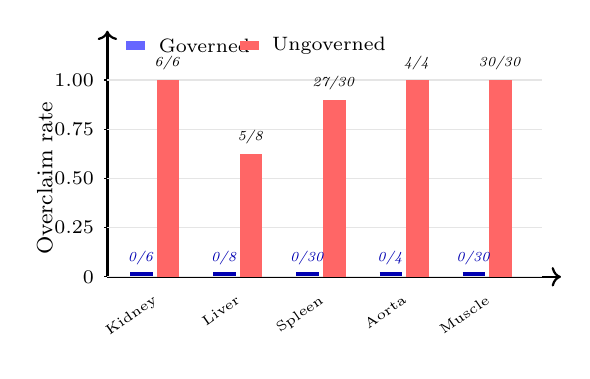
\begin{tikzpicture}[xscale=0.48,yscale=2.5]
  % axes
  \draw[thick,->] (0,0) -- (12,0);
  \draw[thick,->] (0,0) -- (0,1.25);
  % y-axis
  \foreach \y/\lab in {0/0, 0.25/0.25, 0.5/0.50, 0.75/0.75, 1.0/1.00} {
    \draw (0,\y) -- (-0.1,\y) node[left, font=\scriptsize] {\lab};
    \draw[gray!20, thin] (0,\y) -- (11.5,\y);
  }
  \node[rotate=90, font=\footnotesize, anchor=south] at (-1.2, 0.5)
    {Overclaim rate};
  % Kidney (n=6): gov 0%, ungov 100%
  \draw[blue!70!black,very thick] (0.6,0.015) -- (1.2,0.015);
  \fill[red!60] (1.3,0) rectangle (1.9,1.0);
  \node[below, font=\tiny, rotate=35, anchor=north east] at (1.25,-0.02)
    {Kidney};
  \node[above, font=\tiny] at (1.6,1.0) {\textit{6/6}};
  \node[above, font=\tiny, blue!70!black] at (0.9,0.01) {\textit{0/6}};
  % Liver (n=8): gov 0%, ungov 62.5%
  \draw[blue!70!black,very thick] (2.8,0.015) -- (3.4,0.015);
  \fill[red!60] (3.5,0) rectangle (4.1,0.625);
  \node[below, font=\tiny, rotate=35, anchor=north east] at (3.45,-0.02)
    {Liver};
  \node[above, font=\tiny] at (3.8,0.625) {\textit{5/8}};
  \node[above, font=\tiny, blue!70!black] at (3.1,0.01) {\textit{0/8}};
  % Spleen (n=30): gov 0%, ungov 90%
  \draw[blue!70!black,very thick] (5.0,0.015) -- (5.6,0.015);
  \fill[red!60] (5.7,0) rectangle (6.3,0.9);
  \node[below, font=\tiny, rotate=35, anchor=north east] at (5.65,-0.02)
    {Spleen};
  \node[above, font=\tiny] at (6.0,0.9) {\textit{27/30}};
  \node[above, font=\tiny, blue!70!black] at (5.3,0.01) {\textit{0/30}};
  % Aorta (n=4): gov 0%, ungov 100%
  \draw[blue!70!black,very thick] (7.2,0.015) -- (7.8,0.015);
  \fill[red!60] (7.9,0) rectangle (8.5,1.0);
  \node[below, font=\tiny, rotate=35, anchor=north east] at (7.85,-0.02)
    {Aorta};
  \node[above, font=\tiny] at (8.2,1.0) {\textit{4/4}};
  \node[above, font=\tiny, blue!70!black] at (7.5,0.01) {\textit{0/4}};
  % Limb muscle (n=30): gov 0%, ungov 100%
  \draw[blue!70!black,very thick] (9.4,0.015) -- (10.0,0.015);
  \fill[red!60] (10.1,0) rectangle (10.7,1.0);
  \node[below, font=\tiny, rotate=35, anchor=north east] at (10.05,-0.02)
    {Muscle};
  \node[above, font=\tiny] at (10.4,1.0) {\textit{30/30}};
  \node[above, font=\tiny, blue!70!black] at (9.7,0.01) {\textit{0/30}};
  % legend
  \fill[blue!60] (0.5, 1.15) rectangle (1.0, 1.2);
  \node[right, font=\scriptsize] at (1.1, 1.175) {Governed};
  \fill[red!60] (3.5, 1.15) rectangle (4.0, 1.2);
  \node[right, font=\scriptsize] at (4.1, 1.175) {Ungoverned};
  \end{tikzpicture}
  }
\end{figure}

\end{document}
